\documentclass[tikz,border=2pt]{standalone}
\usepackage{amsmath,amssymb}
\usetikzlibrary{arrows.meta}
\begin{document}
% Equivalence principle with E[Z] = 40, E[Y] = 10, E[H] = 5:
% net premium P = 4 balances 4 x 10 = 40 against 40; gross premium 4.5 balances 45 against 40 + 5.
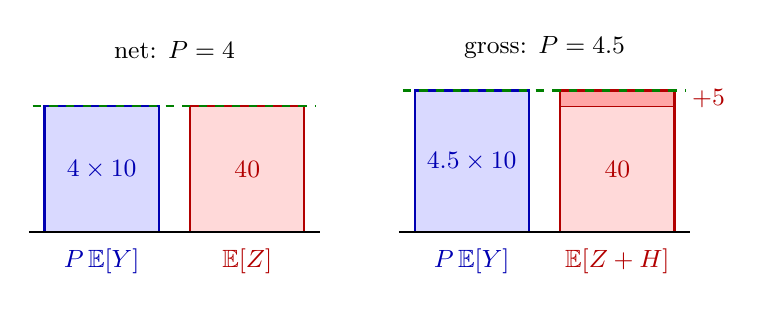
\begin{tikzpicture}[font=\small, >={Latex[length=2mm]}, y=0.04cm]
  \def\bw{1.45}
  % ---- net
  \begin{scope}
    \fill[blue!15] (0,0) rectangle (\bw,40);
    \draw[blue!70!black, thick] (0,0) rectangle (\bw,40);
    \node[blue!70!black, align=center] at (0.5*\bw,20) {$4\times10$};
    \fill[red!15] (1.85,0) rectangle (1.85+\bw,40);
    \draw[red!70!black, thick] (1.85,0) rectangle (1.85+\bw,40);
    \node[red!70!black] at (1.85+0.5*\bw,20) {$40$};
    \draw[green!50!black, thick, dashed] (-0.15,40) -- (2.0+\bw,40);
    \draw[thick] (-0.2,0) -- (2.05+\bw,0);
    \node[blue!70!black, anchor=north] at (0.5*\bw,-2) {$P\,\mathbb E[Y]$};
    \node[red!70!black, anchor=north] at (1.85+0.5*\bw,-2) {$\mathbb E[Z]$};
    \node[anchor=south] at (0.925+0.5*\bw,52) {net: $P=4$};
  \end{scope}
  % ---- gross
  \begin{scope}[xshift=4.7cm]
    \fill[blue!15] (0,0) rectangle (\bw,45);
    \draw[blue!70!black, thick] (0,0) rectangle (\bw,45);
    \node[blue!70!black] at (0.5*\bw,22.5) {$4.5\times10$};
    \fill[red!15] (1.85,0) rectangle (1.85+\bw,40);
    \fill[red!35] (1.85,40) rectangle (1.85+\bw,45);
    \draw[red!70!black, thick] (1.85,0) rectangle (1.85+\bw,45);
    \draw[red!70!black, thin] (1.85,40) -- (1.85+\bw,40);
    \node[red!70!black] at (1.85+0.5*\bw,20) {$40$};
    \node[red!70!black, anchor=west] at (1.95+\bw,42.5) {$+5$};
    \draw[green!50!black, thick, dashed] (-0.15,45) -- (2.0+\bw,45);
    \draw[thick] (-0.2,0) -- (2.05+\bw,0);
    \node[blue!70!black, anchor=north] at (0.5*\bw,-2) {$P\,\mathbb E[Y]$};
    \node[red!70!black, anchor=north] at (1.85+0.5*\bw,-2) {$\mathbb E[Z+H]$};
    \node[anchor=south] at (0.925+0.5*\bw,52) {gross: $P=4.5$};
  \end{scope}
\end{tikzpicture}
\end{document}
